\documentclass[a1paper,fontscale=.47]{baposter}

%%%%lualatex on
%\usepackage{luatextra}
\usepackage{fontspec}
%Ligatures={Contextual, Common, Historical, Rare, Discretionary}
\setmainfont[Mapping=tex-text]{Lora}

%%%lua off
%\usepackage[utf8x]{inputenc}
%\usepackage[T1]{fontenc} 
%\usepackage{lmodern}

\usepackage{enumerate}
\usepackage[english]{babel}
\usepackage{graphicx} %to insert pictures
\usepackage{color} %to set colors
\usepackage{latexsym}
\usepackage{caption}
\usepackage{multicol}
\usepackage{amsmath}

\usepackage{float}
\usepackage{booktabs}

\newcommand{\specialcell}[2][c]{%
  \begin{tabular}[#1]{@{}c@{}}#2\end{tabular}}


\makeatletter
\let\oldabs\abs
\def\abs{\@ifstar{\oldabs}{\oldabs*}}
\let\oldnorm\norm
\def\norm{\@ifstar{\oldnorm}{\oldnorm*}}
\makeatother


%\usepackage[top=1.5cm,bottom=2cm,left=2.5cm,right=2.5cm]{geometry}
%\linespread{1.5}\selectfont



\author{Simon Carrignon}
\definecolor{bordercol}{RGB}{255,255,255}

\definecolor{headercol1}{RGB}{3,51,123}
%\definecolor{bscol}{RGB}{33,57,112}
\definecolor{bscol}{cmyk}{.98,.58,0,.51}
\definecolor{upfcol}{cmyk}{.02,1,.85,.06}
\definecolor{headercol2}{RGB}{255,255,255}
\definecolor{headerfontcol}{RGB}{255,255,255}
\definecolor{boxcolor}{RGB}{255,255,255}
\definecolor{emphcol}{cmyk}{.71,.49,0,.56}

%%% Save space in lists. Use this after the opening of the list %%%%%%%%%%%%%%%%
\newcommand{\compresslist}{
	\setlength{\itemsep}{1pt}
	\setlength{\parskip}{0pt}
	\setlength{\parsep}{0pt}
}

\newcommand{\coloremph}[1]{
	\textcolor{emphcol}{\bf#1}
}


\begin{document}

\begin{poster}{
	borderColor=white,
	headerColorOne=upfcol,
	headerColorTwo=upfcol,
	headerFontColor=headercol2,
	% Only simple background color used, no shading, so boxColorTwo isn't necessary
	boxColorOne=white,
	boxColorTwo=upfcol,
	%roundedheadershape=roundedright,
	headerfont=\Large\sf\bf,
	%textborder=none,
	headerborder=open,
	background=plain,
	bgColorOne=white,
	boxshade,
	grid,
	columns=2
}
{
    eyecatcher andmp
}
{	
    \begin{flushleft}
	\color{upfcol}{Innovation Process and Economic Equilibrium}
    \end{flushleft}
}
{
    \begin{flushleft}
	Simon Carrignon$^{1,2}$, Xavier Rubio-Campillo$^{3}$\\
	{\small $^{1}$Barcelona Supercomputing Center, $^{2}$Universitat Pompeu Fabra, $^{3}$University of Edinburgh,}
    \end{flushleft}
}
{
%\setlength\fboxsep{0pt}
%\setlength\fboxrule{0.5pt}
\vspace{5mm}
\begin{minipage}[l]{14em}
	
\includegraphics[height=4em]{bscLogo.jpg}\\
	\vfill

	
\includegraphics[height=4em]{img/upf_word_imp.jpg}
    \end{minipage}
}

\headerbox{Introduction}{name=introduction,column=0,row=.01}{


Cultural change comprises processes that modify spread of information by social interaction within a population~\cite{boyd_origin_2005} and numerous social scientists are using an evolutionary framework to model this~\cite{henrich_evolution_2003}.

Here we use the \emph{Fitting to Idealized Outcomes} (FIO) method to explore an agent based framework~\cite{carrignon2015modelingthecoevolutionoftradeandcultureinpastsocieties} designed to study the co-evolution of economy and culture. In this framework, economics, is seen as social activity that depends on particular cultural traits: the value attributed to goods used to trade during the economic activity. Multiple cultural processes (innovation, social learning,\ldots) could influence the way those values evolve through space and time leading to different trade dynamics.

The aim of this study is to combine \emph{FIO} with an agent based model to quantify the likelihood of different innovations rate to lead to a General Equilibrium.

}

\headerbox{Method}{name=ud,column=0,below=introduction}{
\subsection*{General Equilibrium}
In economic theory, a \emph{General Equilibrium} (GE) is reached when, given some available quantities of good, consumer and producers agreed on prices that allow both of them to produce, exchange and consume goods of a particular market in such quantities that nothing is missing nor left in the market and consumer are maximising there utilities. 



\subsection*{Agent Based Model}
To test what kind of cultural processes allow the emergence of such GE, we use a model already developed to study the co-evolution of culture and economy. We have already shown that this model leads to clearing market price and optimal utility (cf Fig.~\ref{fig:ratioEvol}) for particular set of parameters. In this model, groups of agents produce, consume and exchange goods then adapt their trading strategy by innovating, or by learning from someone else. Those two later aspects are the cultural ones that we want to consider. Here the learning processes will remain the same --the agents will always tend to copy the best other agents, and we concentrate ourselves on the innovation process.

In the model, it is represent by a probability $\mu$ that one agent randomly change the price he attributes to a good. This probability $\mu$ is what we call the innovation rate: we want to quantify for what range of values this parameter is more likely to allow a GE to appear.

\begin{figure}[H]
	\begin{tabular}{cc}
		\includegraphics[width=.5\textwidth]{img/ClearingPriceDistanceEvolutionForTrade-G3N500.pdf}&
		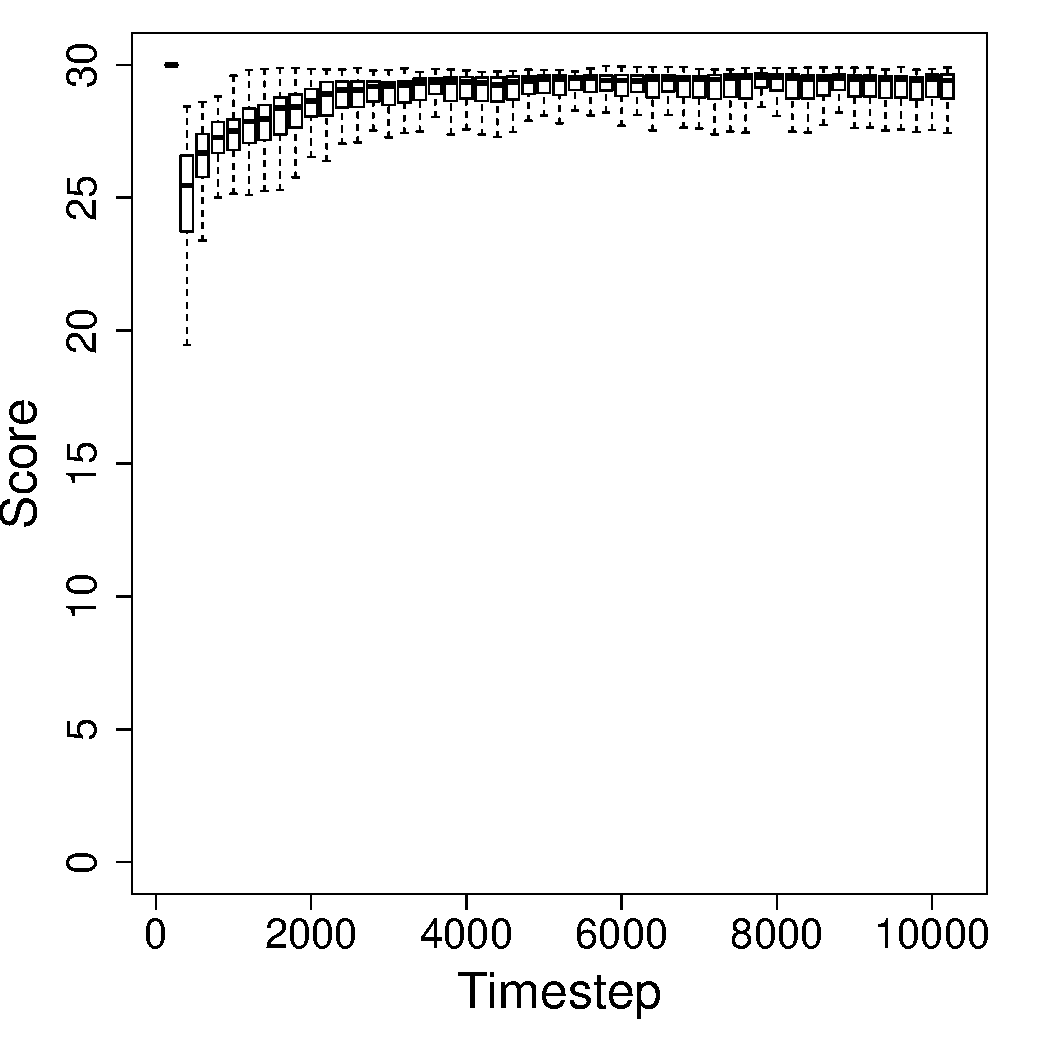
\includegraphics[width=.45\textwidth]{img/ScoreEvolutionForTrade-G3N500.pdf} \\
	\end{tabular}
	\vspace{-.5cm}
	\caption{
	    \small
	    Graphs from \cite{carrignon2015modelingthecoevolutionoftradeandcultureinpastsocieties}, left: evolution of prices toward clearing market prices. Right: evolution of agents score toward the optimal scores.
	}
	\label{fig:ratioEvol}
\end{figure}


\subsection*{Fitting to Idealized Outcomes}

To quantify the likelihood of different assumption on the rate of innovation to lead to a GE we apply a variation of \emph{Approximate Bayesian Computation} (ABC). ABC relies on Bayesian inference to compute and compare the likelihood of models to explain a set of empirical evidence under different parameter distribution. It has been already fruitfully apply to study changes in socio-cultural construct such as battlefield strategies \cite{rubiocampillo2016modelselectioninhistoricalresearchusingapproximatebayesiancomputation}.

Here we use a slight variation of ABC, called \emph{Fitting to Idealized Outcomes} (FIO)~\cite{gallagher2015transitiontofarmingmorelikelyforsmallconservativegroupswithpropertyrightsbutincreasedproductivityisnotessential}, as it compares the parameter space of a model to the output of known theoretical model (instead of empirical evidence).  

\vspace{.2cm}
{
	\footnotesize 
	FIO steps:
\vspace{-.3cm}
\setlength{\columnsep}{1mm}
	\begin{multicols*}{2}
	    \begin{enumerate}
		    \compresslist
		\item sample $\mu$ from uniform distribution ($\mu \sim U(0,1)$)
		\item run simulations with innovation rate = $\mu$ 
		\item compute distance $\epsilon$ to idealize outcome (GE):  
		    \begin{align*}
			\epsilon = \frac{ \sum_{i=1}^{n} s_n-s_{ge} }{n}   
		    \end{align*}
		    {\tiny ($n$: total number of agents, $s_i$ score of agent i, $s_{ge}$: ideal score)}
		    \vfill
		    \columnbreak
		\item select $200$ simulations with $\epsilon<.25$, 
		\item draw \emph{posterior} distribution of $\mu$ for those simulations.
	    \end{enumerate}
	\end{multicols*}
 }

 }




\headerbox{Results}{name=res1,column=1,span=1,row=.01}{

    The Figure~\ref{fig:abc} show the result of the Fitting to Idealized Outcomes. The posterior distribution of the value of $\mu$ used by the best simulation clearly shows that only a restricted range of innovation rate allow the equilibrium to emerge. Without surprise this innovation rate as to be inferior to $0.5$, it would otherwise means that agents are changing their pices almos once every tw time step. This would make any comparison between agents and would prevent any positive change to be fixed in the population.

\begin{figure}[H]
	\centering
		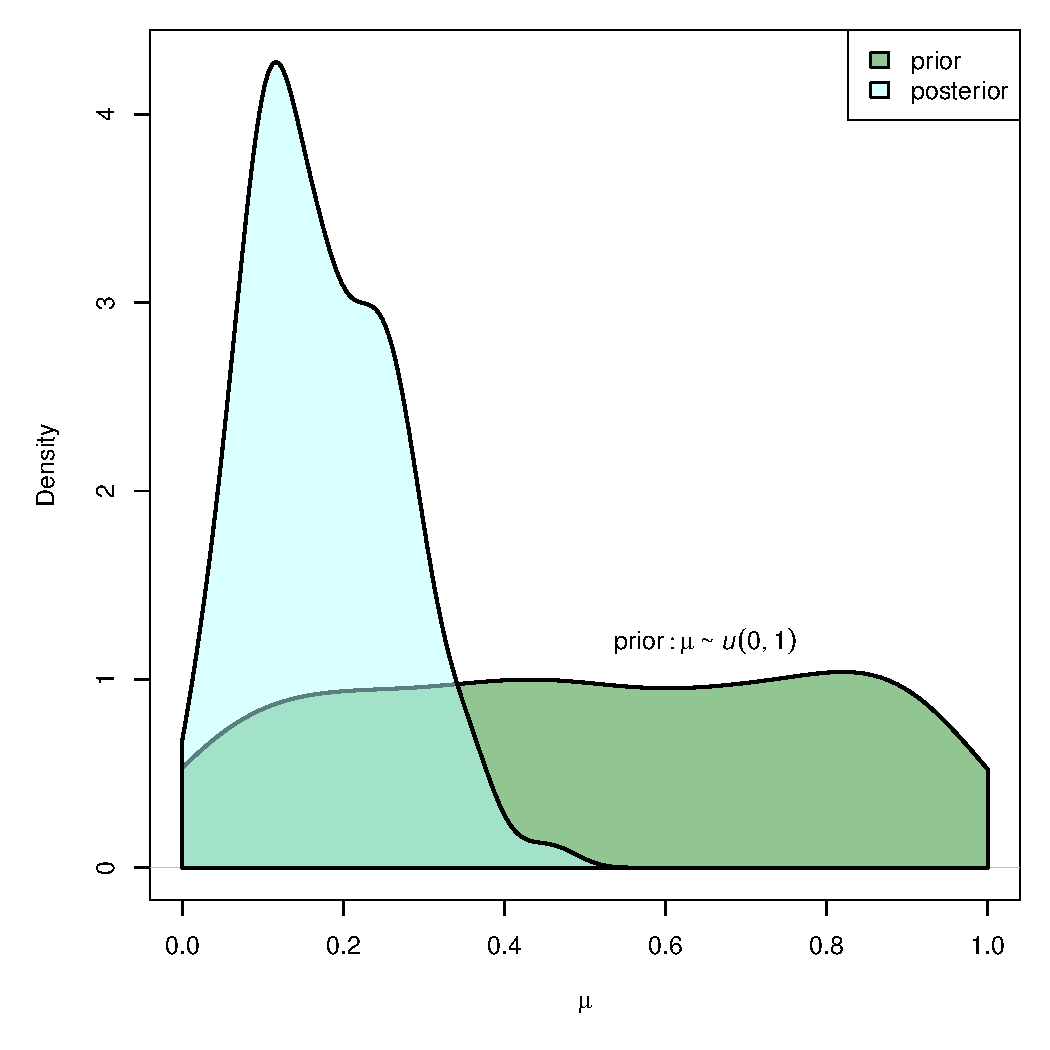
\includegraphics[width=.8\textwidth]{img/ABC.pdf} 
		\vspace{-1cm}
		\caption{\small Result of the FIO: In green the prior distribution where $\mu$ is sampled from. In green the posterior distribution of $\mu$ for the $200$ closest simulation  to the GE. }
		\label{fig:abc}
\end{figure}

On the other hand this innovation rate remains pretty high: the mean value of $\mu$ for the best simulations is $.175$, thus leading to a rate of change of one after 6 time step. If this innovation rate has to be compared to the mutation process acting in biological evolution our result are order of magnitude smaller. This may underlie the difference of speed between biological and social process and the need for the agents to quickly adapt to complex situations.  This could be greatly ameliorate by introducing no-random innovation process and self-adapting strategy such as trial-and-error or more complex experience based learning.

}


\headerbox{Concluding Remarks}{name=conclusion,column=1,below=res1}{

	Though those first result are very limited and concentrated to a simple aspect of the system studied, they show how the use of simulation and model testing tools such as Fitting to Idealize Outcome, can help us to mix different field an. Coupling those result with simple empirical experiment on buisness innovation rate or psychological test on human can be good candidate aorigine apttern shown by model
	
}


\headerbox{References}{name=references,column=1,below=conclusion}{
	\scriptsize
	\renewcommand{\refname}{\vspace{-0.5em}}
	\setlength{\parskip}{0pt}
	\setlength{\itemsep}{0pt}
	\bibliographystyle{abbrv}
	\bibliography{../../biblio/bib/SimonCarrignon,../../biblio/bib/phd,biblio}
}
\headerbox{Acknowledgements}{name=acknowledgements,column=1,below=references}{
    \small
    Funding for this work was provided by the ERC Advanced Grant EPNet (340828).
    \begin{center}
	\includegraphics[width=3cm]{epnetLogo.png}
	\includegraphics[width=2.5cm]{LOGO-ERC.jpg}
    \end{center}
} 

\end{poster}

\end{document}
